\section{Enigma und Turing Bombe}
\label{enigma}
In diesem Abschnitt wird die Enigma und ihre Entschlüsselung thematisiert. Des weiteren wird auf die historischen Hintergründe eingegangen, auf ihre Funktionsweise sowie ihre Fehler.

\subsection{Enigma}
Die Enigma ist eine Verschlüsselungsmaschine, die im zweiten Weltkrieg von den Deutschen genutzt wurde um militärische Fernkommunikation zwischen ihren Truppen zu etablieren. Diese sollte ihnen mit unter einen entschiedenen Vorteil liefern. Dennoch hatte diese Verschlüsselung ein paar sehr große Probleme, die dazu führten, dass die Alliierten immer wieder sehr viele Informationen entschlüsseln konnten.\\
Hauptbestandteile der Enigma waren:
\begin{enumerate}
\item Eingabetastatur
\item Lichtanzeige
\item Steckbrett
\item Reflektor
\item drei oder vier Walzen
\end{enumerate}

\subsubsection{Eingabetastatur}
Eine zur Schreibmaschinen ähnliche Tastatur mit allen 26 Buchstaben des Alphabets, in die man die Nachricht eintippen konnte. Diese Tastatur war mit dem Steckbrett verknüpft.

\subsubsection{Lichtanzeige}
Eine Anzeige mit allen 26 Buchstaben des Alphabets, die einzeln beleuchtet werden und die verschlüsselte Nachricht anzeigen z.B ein H wird eingetippt und ein R wird beleuchtet.

\subsubsection{Steckbrett}
\label{sec:steck}
Das Steckbrett, welches hinten an der Enigma angebracht war, diente zur weiteren Verschlüsselung, da man hier bis zu 13 von 26 Buchstaben manuell miteinander verlinken konnte. Somit wurde z.B. ein eingegebenes A zu einem H und vice versa. Wenn kein Kabel eingesteckt wurde, dann wurde der Buchstabe einfach normal durch geschalltet. Meist wurden nur 10 umgesteckt, da sonst die Anzahl der Möglichkeiten wieder geringer wurden.

\subsubsection{Walzen}
\label{sec:rader}
\begin{wrapfigure}{r}{5cm}

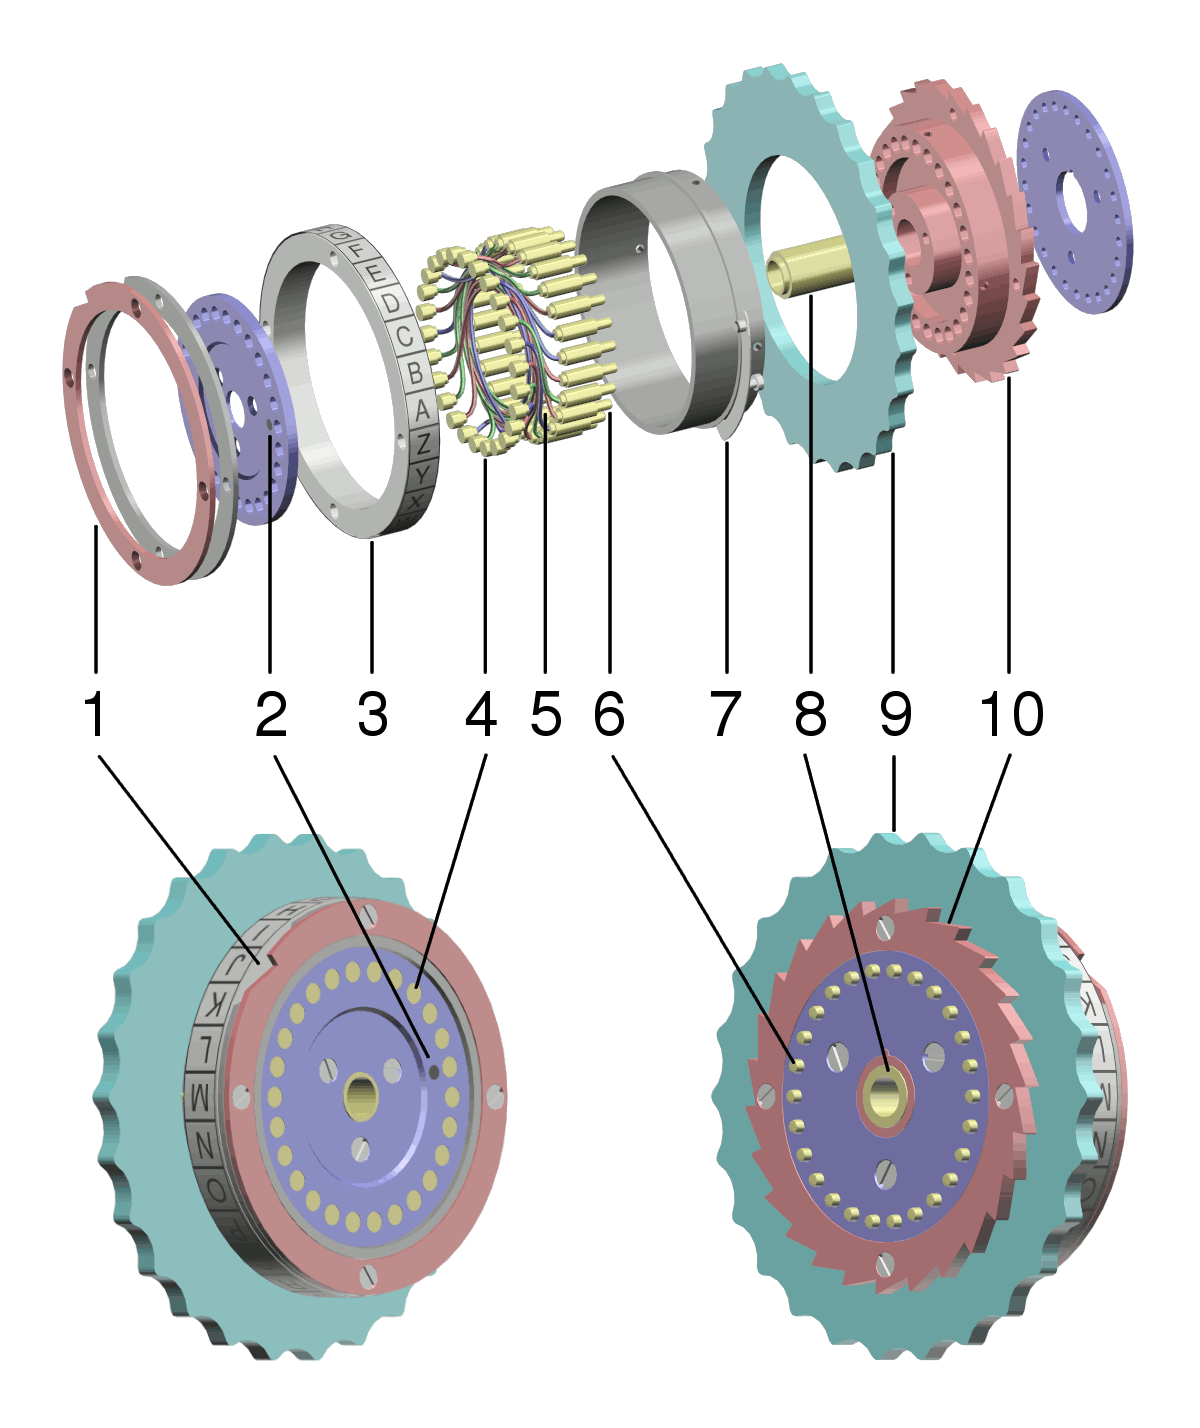
\includegraphics[scale=0.15]{Enigma_rotor_exploded_view.png}
\caption{Walzen Innen}
\label{fig:rotorex}
\end{wrapfigure}
Die Walzen dienten zum weiteren Verschlüsseln der Nachrichten und jeder Walze hatte 26 Stufen für jeden Buchstaben des Alphabets. Wobei das Signal nun innerhalb der Walze durch neue Verkabelung auf einen anderen Buchstaben geleitet wurde (sog. rewiring). Das Signal wurde an die nächste Walze weiter geleitet, dort passiert das selbe nochmal. Es gab 8 verschiedene Arten von Walzen, diese besaßen pro Art immer eine andere Verkabelung innerhalb der Walzen. Walzen der gleichen Art hatten aber immer die selbe Verkabelung. Die erste Walze, welches die Eingabe passierte drehte sich bei jedem Tastendruck um einen Buchstaben weiter. Die nachfolgenden Walzen drehten sich immer dann um eines wenn sich das vorherige an seinem Überrollpunkt befindet. Dieser ist meist wenn sich die Walze einmal um sich selber gedreht hat, dass kann etwa bei M oder aber auch Z sein. Der Überrollpunkt konnte über eine Offset-Markierung an den Walzen eingestellt werden (sog. ring setting), so dass sich die Neuverkabelung um so viele Stellen wie eingestellt in eine Richtung weiter drehten. Diese wurden am Anfang jeder Nachricht einmal eingestellt. Am Anfang wurden diese Starteinstellungen über die Nachricht mitgeteilt, in dem man ein deutsches Wort mit 3 Buchstaben zweimal hintereinander gesendet hat. Was sich jedoch schnell als ziemlich schlechte Idee herausstellte und somit 1938 verboten wurde.

\subsubsection{Reflektor}
Der Reflektor schickte die Signale die von den Rollen kamen durch eine andere Leitung an den Rollen wieder zurück. Dieser konnte nie zum gleichen Buchstaben zurück senden sondern wurde wieder neu verkabelt.

\subsubsection{Beispiel}

\begin{figure}[H]
\centering
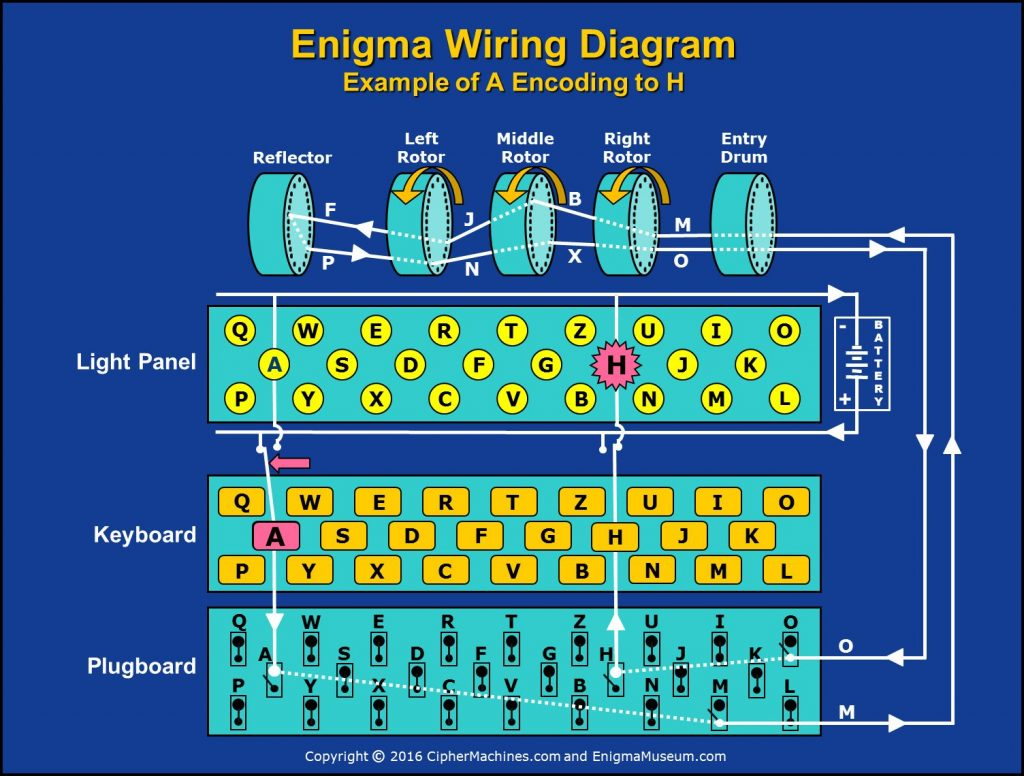
\includegraphics[scale=0.3]{Enigma_Maschine_Beispiel.jpg}
\caption{Beispiel Verkabelung}
\label{fig:enigma}
\end{figure}

Der eingegebene Buchstabe A geht erst einmal an das Steckbrett und ist hier mit dem Buchstaben M verbunden. Dieser wird dann an die Walzen weitergegeben, die den Buchstaben je nach Stellung verändern, hier von M zu B zu J und schließlich zu F. Anschließend wird der Buchstabe wieder zurück durch die Walzen geleitet und kommt in diesem Beispiel als O heraus und wird wieder an das Steckbrett weitergeleitet. Der Buchstabe O ist hier mit H verbunden und so wird am Ende H in der Anzeige beleuchtet, und somit wurde A zu H verschlüsselt.

\subsection{Historie}
Turing beschäftigte sich bereits vor Beginn des zweiten Weltkriegs mit den Enigma Maschinen. Diese waren jedoch von den Italienern und wesentlich simpler als die Enigma Maschinen, die später von den Deutschen eingesetzt wurden. Die erste Version der Enigma war frei verkäuflich und wurde eher privat genutzt da sie nicht viel Sicherheit bot. In dieser Version gab es lediglich 3 der in Sektion \ref{sec:rader} beschriebenen Räder, die in unterschiedlicher Reihenfolge eingesetzt werden konnten. Damit gab es lediglich $3! = 6$ Anordnungsmöglichkeiten. Zu dieser Zeit gab es außerdem kein, wie in Sektion \ref{sec:steck} aufgeführtes Steckbrett. Ein polnisches Verschlüsselungsteam unter der Leitung von Marian Rejewski legte den Grundstein und knackte die Verschlüsselungen der Enigma sehr schnell, dort wurden sie zum ersten mal mit Steckbrett Versionen konfrontiert. Diese knackten sie von Hand mit Hilfe von Lochpapieren. Deutschland wollte sich diese Verschlüsselungsmaschinen nun für militärische Zwecke zu nutzen machen, so entwickelten sie die nächste Version, die militärische Enigma. In dieser Version wurden zwei Walzen zur Auswahl hinzugefügt. Nun wurden also 3 aus 5 Walzen genommen und in unterschiedlichen Anordnungen in der Enigma kombiniert. Diese wurden nachher großflächig für die deutsche Luftwaffe und Armee eingesetzt. Doch der Marine war das nicht genug. Unter Admiral Karl Dönitz wurde eine Enigma speziell für die Marine entwickelt, bei der zu erst 3 aus 8 Walzen und später dann 4 aus 8 Walzen für die Verschlüsselung verwendet wurden. Zu allem Überfluss drehten sich die Räder 6 bis 8 zweimal an ihrem Überrollpunkt. Damit explodierten die möglichen Kombinationen fast exponentiell. Bei Ausbruch des Krieges wurde Turing zusammen mit Neuntausend anderen Spezialisten in den Bletchley Park geholt. Dieser Park wurde zu einer wahren Entschlüsselungsfabrik, in dem später mit Hilfe der \emph{Bombe}, 39 Tausend Enigma Nachrichten im Monat entschlüsselt wurden. Die sogenannte \emph{Bombe} war eine automatisierte Maschine zur Entschlüsselung der Enigma Nachrichten. Diese wurde ursprünglich von den Polen bis zur Invasion entwickelt. Durch die Invasion jedoch übergaben sie die von den Polen \emph{Bomba} genannte Maschine an die Briten. Dort verbesserten sie die Maschine weiter und bauten im Zuge des Krieges zwischen 60 und 100 verschiedene \emph{Bombes} in Großbritannien und noch einmal mindestens so viel in der USA. Dort halfen sie den Briten beim dechiffrieren per Unterseekabel. In Bletchley Park wurde der Platz sehr eng, deswegen wurden um das eigentliche Gebäude mehrere Hütten gebaut, die sogenannten \emph{Huts}. Schnell bekamen die \emph{Huts} spezielle Aufgaben. So war Hut 8, der Arbeitsplatz von Turing, mit der Entschlüsselung der sehr schweren Marine Enigma betraut. Die normalen Enigma Texte der Armee und der Luftwaffe wiederum, wurden in Hut 6 unter der Leitung von Gordon Welchman, ein weiterer berühmter Statistiker, bearbeitet.  \cite{enigmaproblem1} \cite{theessentialturing}

\subsection{Anzahl der Möglichkeiten}
Da die Turing Bombe größtenteils versucht hat den Code durch ausprobieren heraus zu finden, war das schier unmöglich auf Grund der Anzahl an Möglichkeiten. Dennoch konnte man die Anzahl an Möglichkeiten reduzieren (siehe nächstes Kapitel). Hier möchte ich einmal auf die Anzahl der Möglichkeiten bei einer normalen Enigma der Arme eingehen. Dadurch das man 3 aus 5 Rotoren auswählen musste ergibt sich $5 \cdot 4 \cdot 3 = 60$ Möglichkeiten (hier gilt ziehen ohne zurücklegen, da nie zwei Walzen der gleichen Art in der Enigma waren). Dazu kommen noch die Ringeinstellungen. Hier gab es für jede Walze eine Ringeinstellung mit je 26 Möglichkeiten bei 3 Walzen macht $26^3 = 17576$ Möglichkeiten oben drauf. Das schlimmste war jedoch das Steckbrett. Es gibt $!26$ Möglichkeiten Buchstaben mit einander zu kombinieren. Hier wurden jedoch immer nur 20 Buchstaben neu verbunden, somit bleiben 6 übrig also $!6$. Die Ordnung der Verbindungen ist uns egal sowie AB ist das gleiche als BA. Somit gibt es für das Steckbrett $\dfrac{!26}{2^{10}\cdot!6\cdot!10}$ das sind Rund $1.5 \cdot 10^{13}$ Möglichkeiten. Wenn man alle Möglichkeiten zusammen rechnet kommt man auf Rund $1.6 \cdot 10^{20}$  Möglichkeiten\cite{emach}

\subsection{Schwachstellen}
Die Enigma hatte einige Schwachstellen, die im ersten Moment vielleicht nicht als solche erscheinen. Dazu gehörte einmal, dass der Reflektor die Signale nie auf den gleichen Buchstaben zurück leiten konnte. Dadurch konnte man versuchen bekannte Wörter wie zum Beispiel "Wetterbericht" unter den verschlüsselten Text zu halten. Wenn einer der Buchstaben in dem Wort mit dem verschlüsselten Text an der Stelle übereinstimmte, dann konnte es sich nicht um das Wort handeln. Ziel der Entschlüsselung war es heraus zu finden mit welchen der Räder und mit welchen Walzeneinstellungen sie die \emph{Bombe} bestücken mussten. Diese sollte dann automatisch die Nachrichten entschlüsseln. Des weiteren war bei den Rollen 6 bis 8 der Marine das zweite Überrollen ein Indikator dafür, dass eine solche Walze eingesetzt wurde. Dies konnte die Möglichkeiten sehr einschränken. Das oben genannte Problem mit dem doppelt senden eines deutschen Wortes mit 3 Buchstaben hat natürlich dafür gesorgt, dass hier über die Wahrscheinlichkeiten in der Sprache es sehr einfach war die Ringeinstellung zu erraten. Mit Hilfe des oben genannten Reflektor Problems minimierte es natürlich weiter die Möglichkeiten. Dieses Problem bemerkten die Deutschen und verbaten diese Übersendung von Ringeinstellungen. Des weiteren halfen gestohlene Codebücher und Insiderinformationen beim Entschlüsseln. Dazu kam, dass die Deutschen jeden Morgen  um Punkt 6 Uhr ihren Wetterbericht sendeten, denn dieser begann mit dem Wort \emph{Wetterbricht} und endete mit \emph{Heil Hitler}. So konnte man erheblich die Einstellungsmöglichkeiten reduzieren, da man Verbindungen ausschließen konnte.\cite{enigmaflaw} \cite{enigmaproblem1}
\subsubsection{Beispiel}
Man nehme an wir haben den Ausgangstext "wetterberichttesttesttestheilhitler" und geben den in eine Enigma mit den Folgenden Einstellungen ein. \begin{wrapfigure}{r}{5cm}
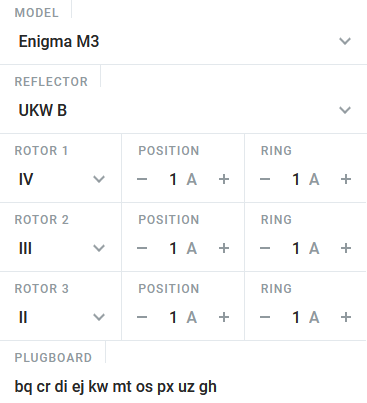
\includegraphics[scale=0.5]{codegen.png}
\caption{Beispiel Enigma Code\cite{encoding}}
\label{fig:ecode}
\end{wrapfigure}
Dann bekommt man folgendes Resultat: "ejzsx opnes prwib kujgg izyac fjpdz hyzsd", wenn man nun versucht immer das Wort Wetterbericht darunter zu legen, kann man ganz schnell mögliche Positionen ausschließen wo das Wort nicht stehen kann.
\begin{table}[H]
\begin{tabular}{|l|l|}
\hline
ejzsxopnesprwibkujggizyacfjpdzhyzsd\\
wetterbericht\\
\hline
ejzsxopnesprwibkujggizyacfjpdzhyzsd\\
$\:$wetterbericht\\
\hline
ejzsxopnesprwibkujggizyacfjpdzhyzsd\\
$\:\:\:$wetterbericht\\
\hline
\end{tabular}
\end{table}
Wie man in der Tabelle sehen kann ist es möglich, dass das Word Wetterbericht als erstes Wort im verschlüsselten Text ist aber nicht an zweiter Stelle, da das dritte E mit dem Code übereinstimmt. Es kann aber wieder an der dritten Stelle stehen, und so weiter. Nun vermuten wir, dass es sich bei dem Text um den Wetterbericht handelt. Ziel ist es nun herauszufinden